\begin{frame}{Progettazione Logica}
Questa operazione si divide in due fasi:
\begin{itemize}[<+->]
    \item \textbf{Ristrutturazione} del modello E-R;
    \item \textbf{Traduzione} verso il modello logico.
\end{itemize}
\end{frame}
%
\begin{frame}{Ristrutturazione}
    La ristrutturazione serve a rendere il diagramma E-R pi\`u versatile alle esigenze dell`utente e per rimuovere eventuali errori di progettazione. Si divide in 5 fasi.
    \uncover<2->{\\\vspace{1em} Per questa operazione bisogna tenere da conto i 4 indici del \textbf{carico applicativo}:}
    
    \begin{columns}
        \begin{column}{0.6\textwidth}
            \uncover<2->{\begin{itemize}
                \item costo di un`operazione
                \item occupazione di memoria
                \item volume dati
                \item caratteristiche delle operazioni
            \end{itemize}}
        \end{column}
        \begin{column}{0.4\textwidth}
            \uncover<3->{\only<3>{\\\texttt{\textcolor{red}{Questi sono parametri da
                tenere da conto per progetti
                veri e propri, solo dopo aver
                effettuato un`approfondita
                ingegnerizzazione.}}
            }\only<4>{\texttt{\textcolor{red}{Per un esame scritto questi parametri non hanno significato, basta quindi appellarsi al buon senso.}}
            }}
        \end{column}
    \end{columns}
\end{frame}
%
\begin{frame}{Ristrutturazion: Fase 1}
\textbf{1) Analisi delle ridondanze}
\\\vspace{2em}
In uno schema ER le ridondanze sono le presenze ripetute di attributi che possono essere ricavate da altri.
    \only<2>{\begin{figure}[h]
        \centering
        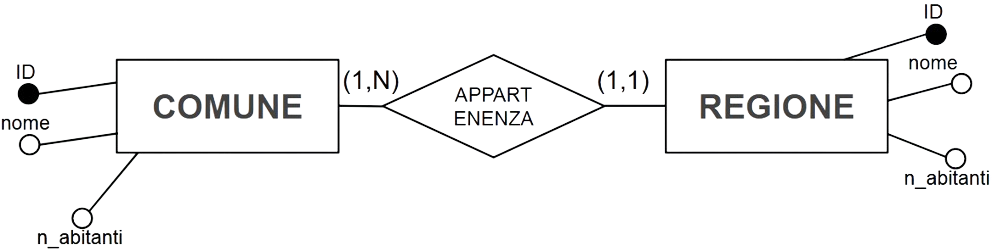
\includegraphics[width=0.7\textwidth]{img/i1.png}
    \end{figure}}
    \only<3>{\begin{figure}[h]
        \centering
        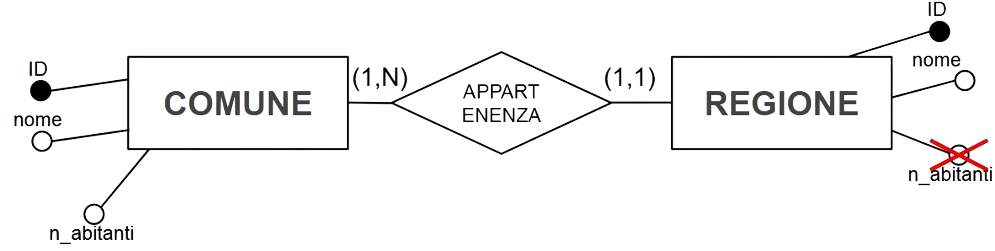
\includegraphics[width=0.7\textwidth]{img/i2.png}
    \end{figure}}
    \only<4>{\begin{figure}[h]
        \centering
        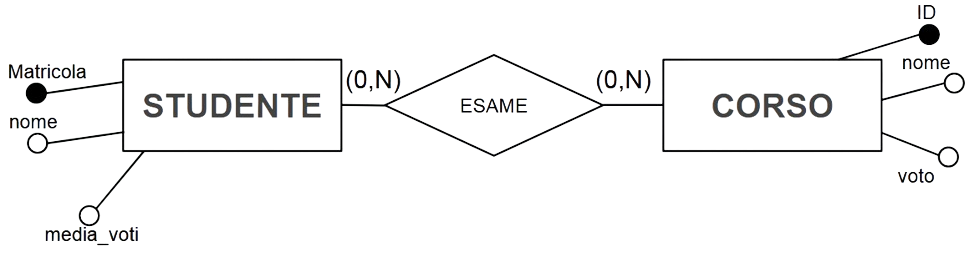
\includegraphics[width=0.7\textwidth]{img/i3.png}
    \end{figure}}
    \only<5>{\begin{figure}[h]
        \centering
        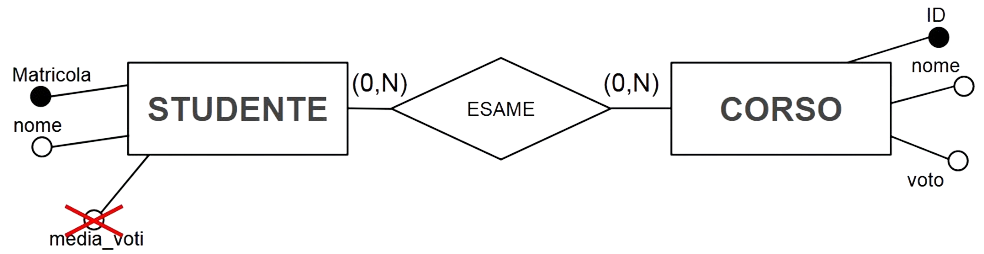
\includegraphics[width=0.7\textwidth]{img/i4.png}
    \end{figure}}
\end{frame}
%
\begin{frame}{Ristrutturazion: Fase 2}
\textbf{2) Partizionamento/accorpamento di entit\`a e associazioni}
\\\vspace{2em}
Gli accessi ad una entit\`a possono essere ridotti separando o raggruppando degli attributi.
\begin{figure}[h]
        \centering
        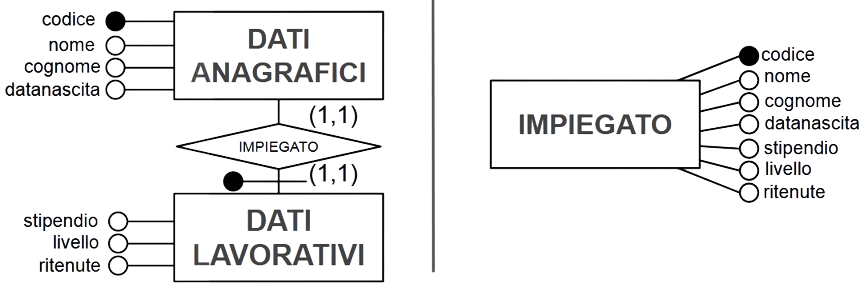
\includegraphics[width=0.8\textwidth]{img/i5.png}
    \end{figure}
\end{frame}
%
\begin{frame}{Ristrutturazion: Fase 3}
\textbf{3) Eliminazione delle generalizzazioni}
\\\vspace{2em}
Il modello logico del DB non permette la presenza di generalizzazioni, vanno quindi eliminate. Ci sono 3 diversi metodi di eliminazione e vanno scelti in base alle esigenze.
\begin{figure}[h]
        \centering
        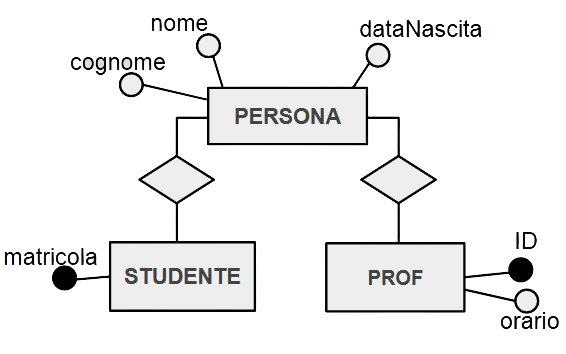
\includegraphics[width=0.5\textwidth]{img/i6.png}
    \end{figure}
\end{frame}
%
\begin{frame}{Ristrutturazione}
\textbf{3) Eliminazione delle generalizzazioni}
\\\vspace{2em}
\begin{center}
    \textbf{MANTENIMENTO DELLE ENTIT\`A CON ASSOCIAZIONI}
\end{center}
\begin{columns}
        \begin{column}{0.5\textwidth}
            \begin{figure}[h]
        \centering
        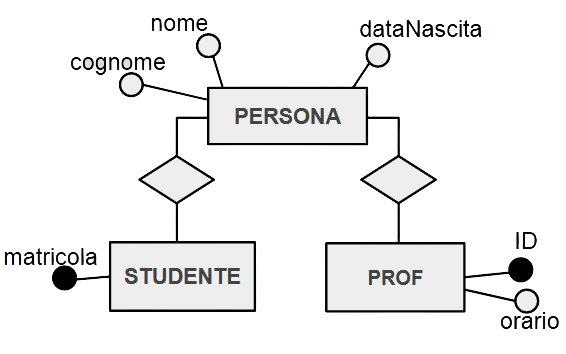
\includegraphics[width=1\textwidth]{img/i6.png}
    \end{figure}
        \end{column}
        \begin{column}{0.5\textwidth}
            \begin{figure}[h]
        \centering
        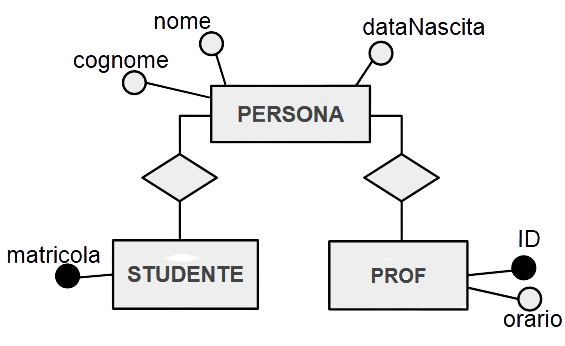
\includegraphics[width=1\textwidth]{img/i7.png}
    \end{figure}
        \end{column}
    \end{columns}
\end{frame} 
%
\begin{frame}{Ristrutturazion: Fase 3}
\textbf{3) Eliminazione delle generalizzazioni}
\\\vspace{2em}
\begin{center}
    \textbf{COLLASSO VERSO L`ALTO}
\end{center}
\begin{columns}
        \begin{column}{0.5\textwidth}
            \begin{figure}[h]
        \centering
        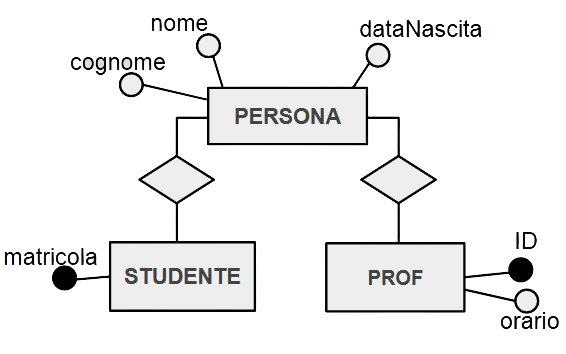
\includegraphics[width=1\textwidth]{img/i6.png}
    \end{figure}
        \end{column}
        \begin{column}{0.5\textwidth}
            \begin{figure}[h]
        \centering
        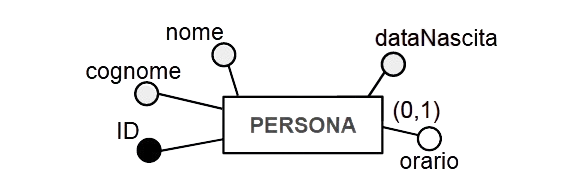
\includegraphics[width=1\textwidth]{img/i8.png}
    \end{figure}
        \end{column}
    \end{columns}
\end{frame}
%
\begin{frame}{Ristrutturazion: Fase 3}
\textbf{3) Eliminazione delle generalizzazioni}
\\\vspace{2em}
\begin{center}
    \textbf{COLLASSO VERSO IL BASSO}
\end{center}
\begin{columns}
        \begin{column}{0.5\textwidth}
            \begin{figure}[h]
        \centering
        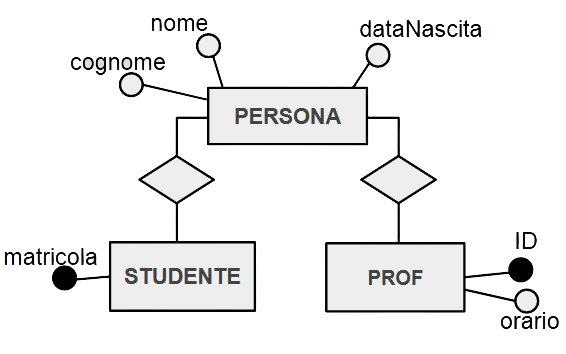
\includegraphics[width=1\textwidth]{img/i6.png}
    \end{figure}
        \end{column}
        \begin{column}{0.5\textwidth}
            \begin{figure}[h]
        \centering
        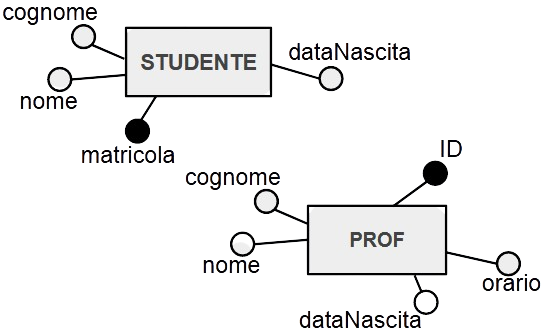
\includegraphics[width=0.9\textwidth]{img/i9.png}
    \end{figure}
        \end{column}
    \end{columns}
\end{frame}
%
\begin{frame}{Ristrutturazion: Fase 4}
\vspace{-3cm}
\textbf{4) scelta degli identificatori primari}
\\\vspace{2em}
Le chiavi primarie devono essere non nulle e non esterne. Sono da preferire chiavi non composte o almeno composte da meno attributi possibile.
\end{frame}
%
\begin{frame}{Ristrutturazion: Fase 5}
\textbf{5) Normalizzazione degli attributi}
\\\vspace{2em}
Gli attributi composti devono essere rimossi.
\begin{columns}
        \begin{column}{0.5\textwidth}
            \begin{figure}[h]
        \centering
        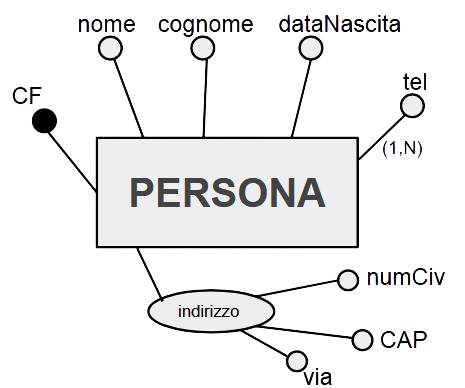
\includegraphics[width=0.75\textwidth]{img/i10.png}
    \end{figure}
        \end{column}
        \begin{column}{0.5\textwidth}
        \uncover<2->{\only<2>{\begin{figure}[h]
        \centering
        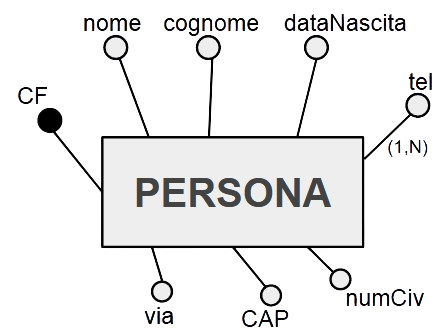
\includegraphics[width=0.8\textwidth]{img/i11.png}
    \end{figure}}
    \only<3>{\begin{figure}[h]
        \centering
        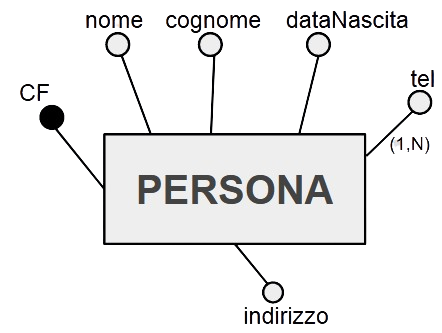
\includegraphics[width=0.8\textwidth]{img/i12.png}
    \end{figure}}}
        \end{column}
    \end{columns}
\end{frame}
%
\begin{frame}{Ristrutturazion: Fase 5}
\textbf{5) Normalizzazione degli attributi}
\\\vspace{2em}
Gli attributi con cardinalit\`a devono essere trasformati in entit\`a
\begin{columns}
        \begin{column}{0.5\textwidth}
            \begin{figure}[h]
        \centering
        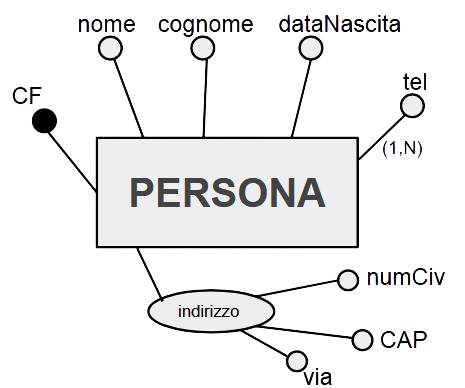
\includegraphics[width=0.75\textwidth]{img/i10.png}
    \end{figure}
        \end{column}
        \begin{column}{0.5\textwidth}
        \uncover<2->{\begin{figure}[h]
        \centering
        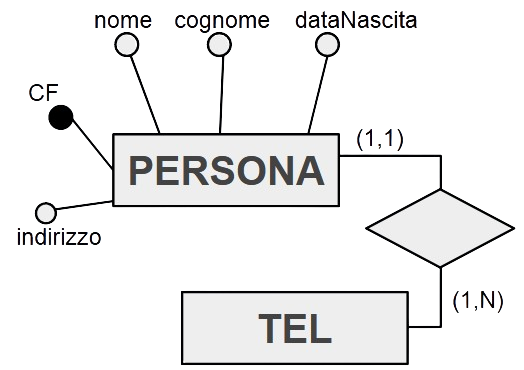
\includegraphics[width=0.8\textwidth]{img/i13.png}
    \end{figure}}
        \end{column}
    \end{columns}
\end{frame}
%
\begin{frame}{Traduzione}
\textbf{associazione uno-a-uno}
    \begin{figure}[h]
        \centering
        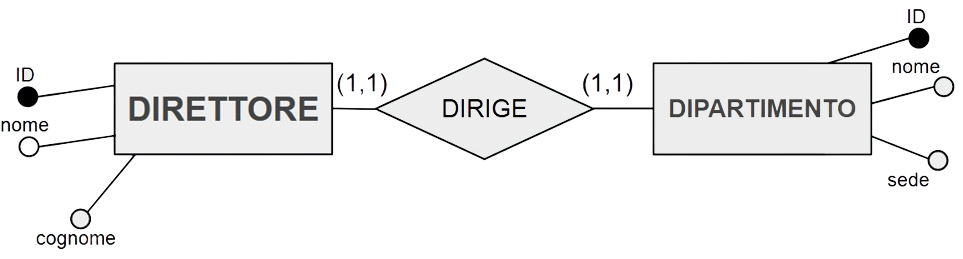
\includegraphics[width=0.8  \textwidth]{img/i14.png}
    \end{figure}
\begin{center}
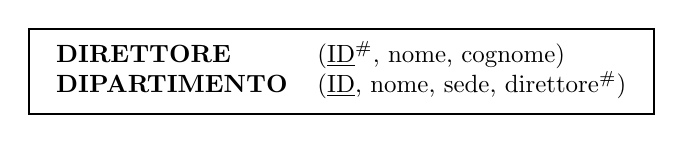
\begin{tikzpicture}
    \node[draw=black, thick, inner sep=5pt, scale=0.9] {
        \begin{tabular}{ll}
            \textbf{DIRETTORE} & (\underline{ID}$^{\#}$, nome, cognome) \\
            \textbf{DIPARTIMENTO} & (\underline{ID}, nome, sede, direttore$^{\#}$)
        \end{tabular}
    };
\end{tikzpicture}
\vspace{0.3cm}

\uncover<2->{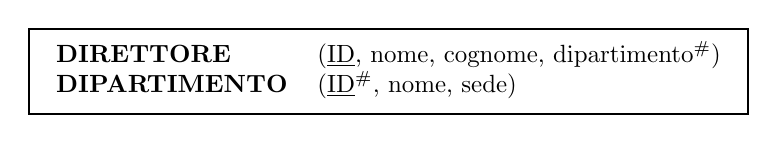
\begin{tikzpicture}
    \node[draw=black, thick, inner sep=5pt,scale = 0.9] {
        \begin{tabular}{ll}
            \textbf{DIRETTORE} & (\underline{ID}, nome, cognome, dipartimento$^{\#}$) \\
            \textbf{DIPARTIMENTO} & (\underline{ID}$^{\#}$, nome, sede)
        \end{tabular}
    };
\end{tikzpicture}}
\end{center}
\end{frame}
%
\begin{frame}{Traduzione}
\textbf{associazione uno-a-uno}
    \begin{figure}[h]
        \centering
        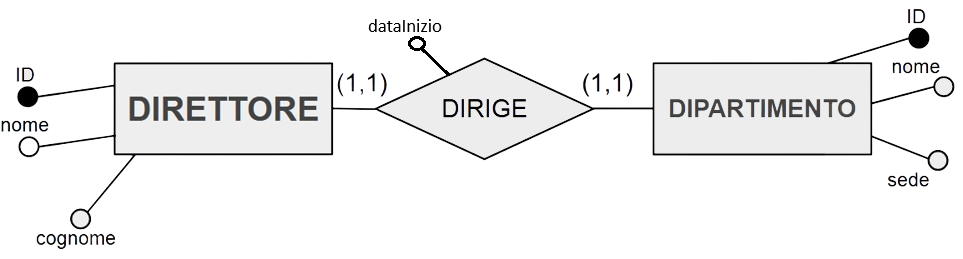
\includegraphics[width=0.8  \textwidth]{img/i14_2.png}
    \end{figure}
\begin{center}
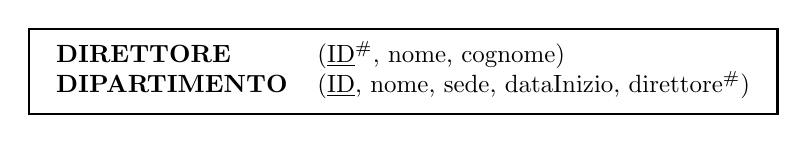
\begin{tikzpicture}
    \node[draw=black, thick, inner sep=5pt, scale=0.9] {
        \begin{tabular}{ll}
            \textbf{DIRETTORE} & (\underline{ID}$^{\#}$, nome, cognome) \\
            \textbf{DIPARTIMENTO} & (\underline{ID}, nome, sede, dataInizio, direttore$^{\#}$)
        \end{tabular}
    };
\end{tikzpicture}
\vspace{0.3cm}

\uncover<2->{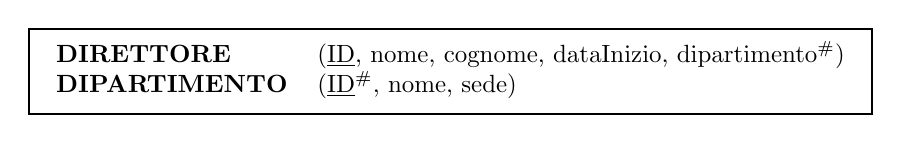
\begin{tikzpicture}
    \node[draw=black, thick, inner sep=5pt,scale = 0.9] {
        \begin{tabular}{ll}
            \textbf{DIRETTORE} & (\underline{ID}, nome, cognome, dataInizio, dipartimento$^{\#}$) \\
            \textbf{DIPARTIMENTO} & (\underline{ID}$^{\#}$, nome, sede)
        \end{tabular}
    };
\end{tikzpicture}}
\end{center}
\end{frame}
%
\begin{frame}{Traduzione}
\textbf{associazione uno-a-molti (attributo su relazione)}
    \begin{figure}[h]
        \centering
        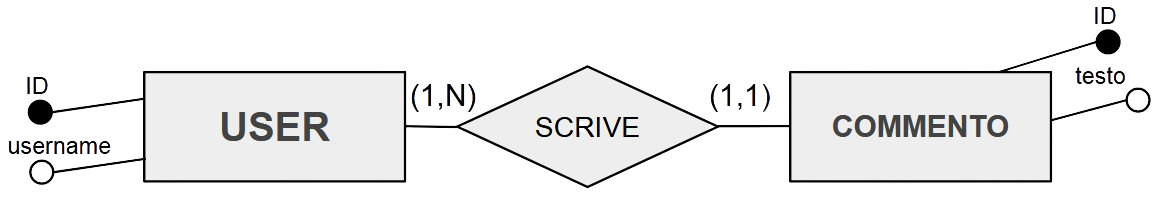
\includegraphics[width=0.8  \textwidth]{img/i15.png}
    \end{figure}
    \vspace{0.8cm}
\uncover<2->{\begin{center}
    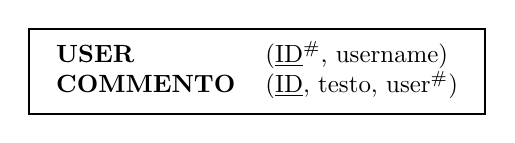
\begin{tikzpicture}
    \node[draw=black, thick, inner sep=5pt, scale=0.9] {
        \begin{tabular}{ll}
            \textbf{USER} & (\underline{ID}$^{\#}$, username) \\
            \textbf{COMMENTO} & (\underline{ID}, testo, user$^{\#}$)
        \end{tabular}
    };
\end{tikzpicture}
\end{center}}
\end{frame}
%
\begin{frame}{Traduzione}
\textbf{associazione uno-a-molti}
    \begin{figure}[h]
        \centering
        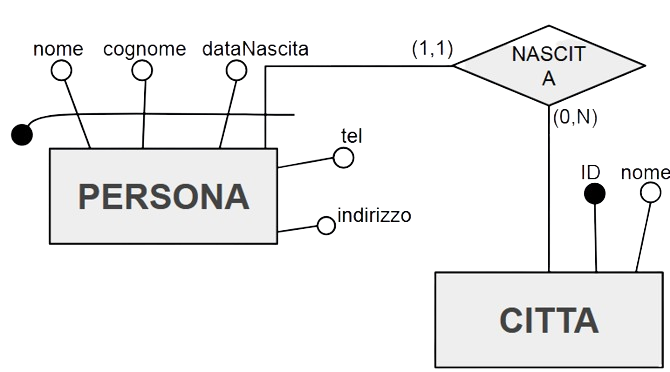
\includegraphics[width=0.5  \textwidth]{img/i16.png}
    \end{figure}
    \vspace{0.5cm}
\uncover<2->{
\begin{center}\only<2>{
    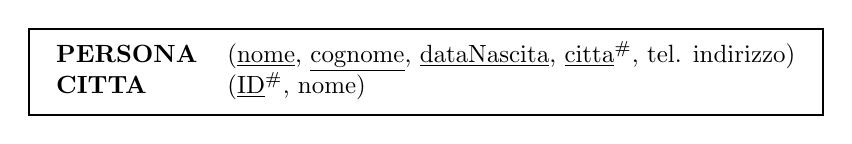
\begin{tikzpicture}
    \node[draw=black, thick, inner sep=5pt, scale=0.9] {
        \begin{tabular}{ll}
            \textbf{PERSONA} & (\underline{nome}, \underline{cognome}, \underline{dataNascita}, \underline{citta}$^{\#}$, tel. indirizzo) \\
            \textbf{CITTA} & (\underline{ID}$^{\#}$, nome)
        \end{tabular}
    };
\end{tikzpicture}}
\only<3>{
    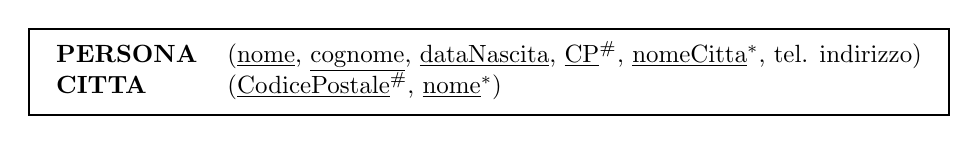
\begin{tikzpicture}
    \node[draw=black, thick, inner sep=5pt, scale=0.9] {
        \begin{tabular}{ll}
            \textbf{PERSONA} & (\underline{nome}, \underline{cognome}, \underline{dataNascita}, \underline{CP}$^{\#}$, \underline{nomeCitta}$^{*}$, tel. indirizzo) \\
            \textbf{CITTA} & (\underline{CodicePostale}$^{\#}$, \underline{nome}$^{*}$)
        \end{tabular}
    };
\end{tikzpicture}}
\end{center}}
\end{frame}
%
\begin{frame}{Traduzione}
\textbf{associazione molti-a-molti}
\begin{figure}[h]
        \centering
        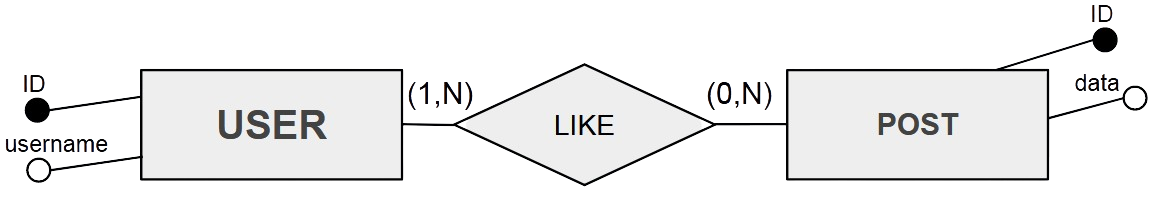
\includegraphics[width=1  \textwidth]{img/i17.png}
\end{figure}
\vspace{0.8cm}
\begin{center}
\uncover<2->{
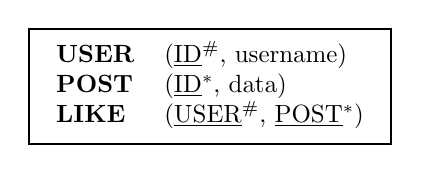
\begin{tikzpicture}
    \node[draw=black, thick, inner sep=5pt, scale=0.9] {
        \begin{tabular}{ll}
            \textbf{USER} & (\underline{ID}$^{\#}$, username) \\
            \textbf{POST}& (\underline{ID}$^*$, data)\\
            \textbf{LIKE} & (\underline{USER}$^{\#}$, \underline{POST}$^{*}$)
        \end{tabular}
    };
\end{tikzpicture}}
\end{center}
\end{frame}
%
\begin{frame}{Traduzione}
\textbf{associazione molti-a-molti(ricorsiva)}
\begin{figure}[h]
        \centering
        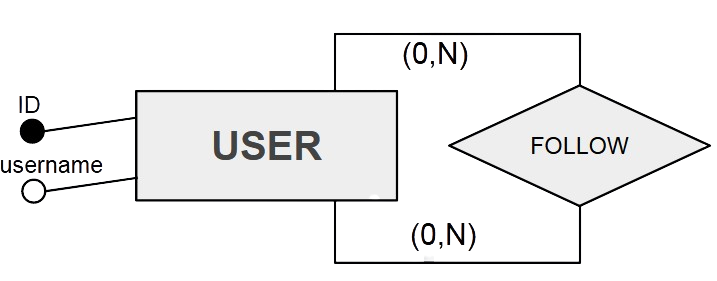
\includegraphics[width=0.7  \textwidth]{img/i18.png}
\end{figure}
\vspace{0.5cm}
\begin{center}
\uncover<2->{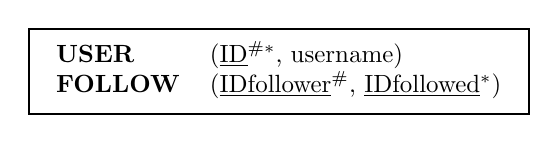
\begin{tikzpicture}
    \node[draw=black, thick, inner sep=5pt, scale=0.9] {
        \begin{tabular}{ll}
            \textbf{USER} & (\underline{ID}$^{\#*}$, username) \\
            \textbf{FOLLOW}& (\underline{IDfollower}$^\#$, \underline{IDfollowed}$^*$)\\
        \end{tabular}
    };
\end{tikzpicture}}
\end{center}
\end{frame}